\documentclass[fleqn,10pt]{physiome}
% Use option lineno for line numbers 

\articletype{Original}
%% Choose from Original, Retrospective, Review, Letter

\title{A theoretical model of slow wave regulation using voltage-dependent synthesis of inositol 1, 4, 5-trisphosphate}


\author[1][l.noroozbabaee @auckland.ac.nz]{Leyla Noroozbabaee}
\author[3]{Mohammad Imtiaz} 
\author[2]{Dirk Van Heldenn}
\author[1]{Peng Du}
\author[1]{David P. Nickerson} 

\affil[1]{Auckland Bioengineering Institute, University of Auckland, New Zealand}
\affil[2]{School of Biomedical Sciences and Pharmacy, University of Newcastle, Australia}
\affil[3]{Department of Electrical and Computer Engineering, Bradley University,United States}
%% The following lines can be omitted when submitting;
%% information will be added by editors
\publicationdate{20 Jan 2023}
\editor{Karin Lundengård}
\curator{Weiwei Ai}
\submitteddate{4 Sept 2022}
\citethisas{Noroozbabaee et al. (2023)\\A theoretical model of slow wave regulation using voltage-dependent synthesis of inositol 1, 4, 5-trisphosphate. Physiome.}{10.36903/physiome.21708176}
\begin{document}

\maketitle
\begin{abstract}
The system of equations and figures presented in \citet{imtiaz2002theoretical} are verified and reproduced in the current curation paper. Here, to demonstrate reproducibility, We describe the model encoded in the CellML and document the differences between our curated model and the one published by \citeauthor{imtiaz2002theoretical}. From the primary publication, we extracted data applying the Engauge digitizer software \citep{mark_mitchell_2020_3941227} to compare the current CellML simulation results against those in the primary publication.

 
\end{abstract}

\keywords{OpenCOR, Computational model, IP$_{3}$ oscillations, Slow wave, CellML, Membrane potential, Feedback}

\primarypubs[10.36903/physiome.21708176]{Ref}{imtiaz2002theoretical}

\section{Introduction}
Slow waves are rhythmic bioelectrical depolarizations that
initiate and control the mechanical activity of gastrointestinal (GI) smooth
muscles. One of the mechanisms responsible for generating slow waves involves IP$_{3}$-induced calcium release and calcium-induced calcium release from IP$_{3}$-operated intracellular calcium stores. The resultant calcium increases in the subplasmalemmal space then activate calcium-sensitive inward currents across the plasmalemma that result in slow-wave
depolarizations \citep{dicker2018global,imtiaz2002theoretical}.

According to \citet{imtiaz2002theoretical}, IP$_{3}$ oscillations are unnecessary
for calcium oscillations, as IP$_{3}$ oscillations can occur in many different cell types. In the current work \citet{imtiaz2002theoretical}, the authors are introducing a new feedback mechanism based on membrane potential, which then modulates IP$_{3}$ synthesis. Where the aim is to study the role of membrane
potential feedback on IP$_{3}$ synthesis and its role in regulating calcium release and slow waves. The system is simplified by considering a single
isopotential cell with a single IP$_{3}$ receptor-operated intracellular
calcium pool. The ryanodine receptor is ignored in the model. It is
important to note that the voltage-dependent channels are considered to be blocked.

A persistent workspace for this work is available in the Physiome Model Repository at \url{https://models.physiomeproject.org/workspace/763}. The specific version of this implementation used to produce the results presented here is included in the OMEX Archive \citep{bergmann_combine_2014} for this article.

This implementation includes the Python source code to generate the model simulations in a 'Simulations' directory. The corresponding CellML implementation is available in a 'Experiments' directory containing the encoded mathematical model. This CellML file does not reproduce the figures due to limited solver capabilities at the time of testing. As such, we have elected to describe the required simulation experiments in Python and use the OpenCOR \citep{garny_opencor:_2015} Python interpreter to perform the simulations and analyses. In this manuscript, we focus on reproducibility and reusability. 


\section{Model description}
\subsection{Primary Publication}
The model was formulated using a Hodgkin-Huxley type formulation. The cell membrane lipid bilayer was modelled as a capacitance (C$_{m}$),
and the ion channels in the membrane were represented as conductance. The change in the transmembrane potential (V$_{m}$) over time depended on the sum of the individual ion currents in the cell:
\begin{equation}
\frac{dV_{m}}{dt} = - \frac{I_{tot}}{C_{m}}.   
\end{equation}



\subsection{Model Implementation}
The implementation of the model was performed using CellML \citep{doi:10.1177/0037549703040939}. Some simulation values stated in \citet{imtiaz2002theoretical} resulted in different model behaviour, which we adjusted as outlined in \autoref{tab:Inconsistency}. The simulation experiments presented here were performed using OpenCOR (Snapshot 2021-10-5 \citep{garny_opencor:_2015}). Simulation settings and detailed solver information were encoded in SED-ML ducument \citep{waltemath2011reproducible}. 

We reproduced the data represented in \citet[Figures 2A, 3A, 4A, 6(A and B) \& 8A ]{imtiaz2002theoretical} by using different settings corresponding to the various model experiments. We implemented the model configuration in Python scrip for each experiment. Then, we perform the Python script to plot the related data.

The name of the simulation and plot scripts indicates the figure number in the primary paper. For example,
\texttt{Fig2\_sim.py} is used to generate the simulation data, and \texttt{Plot\_Fig2.py} reproduces the graph shown in Figure 2A from \citep{imtiaz2002theoretical}.

\subsection{Model Modifications }
\label{Parameter_Values}

Mathematical Equations were the same as reported in the primary publication of \citet{imtiaz2002theoretical} except for \cite[Equations 3, 7, and 9]{imtiaz2002theoretical}. Please see the correction in below:


\begin{enumerate}

\item Unit consistency:
\begin{enumerate}
\item In Eq. 7, the first term, which indicates the lump current ($I_{i}$) should carry a negative sign, while in the original work, the lump current is presented with a positive sign. 

\item In Eq. 7, we correct the consistency in time unit by multiplying the denominator on the right-hand side by the scale factor of 60 s
\begin{equation*}
\frac{dV_{m}}{dt} = - \Big[\frac{I_{Ca}+ I_{i}-I_{inj}}{C_{m}*60}\Big].
\end{equation*}
\item In Eq. 9,  the term $\beta$ indicates the external stimuli has a unit of $\mu M $ while the term $dP /dt$ which indicates IP$_{3}$ concentration in the cytosol has a unit of $\mu M /min$.
The baseline parameter values are provided in the primary paper \citet{imtiaz2002theoretical}.
\begin{equation*}
  \frac{dP}{dt} = \beta - \epsilon *  P  - V_{m4}(P) + P (V)
\end{equation*}



\begin{table}
\centering
\caption{Correction of primary \cite[Tables 1,2 \& 3]{imtiaz2002theoretical}}
\label{tab:Inconsistency}

\begin{tabular}{lccc}

\toprule
Table & Parameter & Primary paper & CellML \\
\midrule

Table 1 & $ V_{1}$ & $3.4 \ \mu M /min$ & $3.4\ 1 /min$ \\
Table 3 & $\beta$ & $0.7 \ \mu M $ &  $0.7 \ \mu M /min$  \\

\bottomrule
\end{tabular}
\end{table}
 \end{enumerate}

\item No initial condition was defined in the primary paper, all initial conditions extracted from the original paper, using Engauge Digitizer software \citep{mark_mitchell_2020_3941227}.

\begin{table}[hbt!]

\centering
\caption{Initial conditions on the current CellML implementations.}\label{tab:Fig3}
\begin{tabular}{lllll}\hline

$V_{m(init)}[mV]$ & $Z_{init}$ & $Y_{init}$ & $P_{IP_{3}}$ & $b_{IP_{3}}$\\ \hline
-65.00 & 4.113 & 0.478 & 0.408 & 0.7533\\
\end{tabular}
\end{table}

\item  In the case of model experiments and simulations, there was no clear information about the protocol details they used to inject the current (stimulus) into the cell. The simulation experiments we have inferred from the primary paper in order to reproduce the simulation results are described in \autoref{Model Simulations}. 

\end{enumerate}

\subsection{Model Simulations}
\label{Model Simulations}
In the presented figures, the dots denote the simulated data extracted from the primary publication, while the solid lines are the simulation results produced by the current CellML implementation.


Figure 3A was reproduced applying the following protocols \autoref{eq:simu2}, while the initial conditions were the same as \autoref{tab:Fig3}.


\begin{equation}
  I_{inject} =
 \begin{cases}
 2.25\ mA  \  \ \   30\ min\ < \ time \ <= \ 31.5\ min\  \\
 2.25\ mA  \  \ \   60\ min\ < \ time \ <= \ 63\ min\ 
 \label{eq:simu2}

  \end{cases}
\end{equation}

Figure 4A was reproduced using the IP$_{3}$ model by setting the initial membrane potential (V$_{m}$) at a fixed holding potential -65.09 mV and then polarizing the membrane by injecting the current into the cell, for more details information see \autoref{eq:simu3} and \autoref{fig:fig4}. 

\begin{equation}
  I_{inject} =
  \begin{cases}
  0\ mA  \  \ \  \ \ \  0\ min\ < \ time \ <= \ 12\ min\  \\
 -15 \ mA  \  \ \   12\ min\ < \ time \ <= \ 24\ min\ \\
 +22 \ mA  \  \ \   24\ min\ < \ time \ <= \ 36\ min 
 \label{eq:simu3}

  \end{cases}
\end{equation}
In Figure 8A, the effect of the interpulse duration on current pulse-induced responses was studied. The aim was to demonstrate the pulse would fail to evoke responses if the interpulse duration was reduced below a critical value. In Fig 8A $t_{d} = 5.36 \ min$, while in Fig 8B $t_{d} = 2.36 \ min$.


\begin{equation}
  I_{inject} =
  \begin{cases}
  0\ mA  \  \ \   5.36\ min\ < \ time   \\
  2 \ mA  \  \ \   5.36 + n*t_{d}\ min\ < \ time \ <= \ 5.36 + n*(t_{d}+0.64)\ min\ 
 \label{eq:simu8} 

  \end{cases}
\end{equation}

\subsection{Model Results}
We employed Engauge Digitizer software \citep{mark_mitchell_2020_3941227} to extract data from all figures from  \citet{imtiaz2002theoretical} to present alongside the results of the present work. The reproduction of all figures of \citet{imtiaz2002theoretical} is given in Figures 1-5, which show good agreement with the data of the primary paper. Solid lines show the output from the current curation, and crosses show discrete points found by the Engauge Digitizer of the figures originally published article.

Applying some corrections to the original equations and parameters (see model modifications), the following results were produced:

\begin{figure}[ht!]%\centering
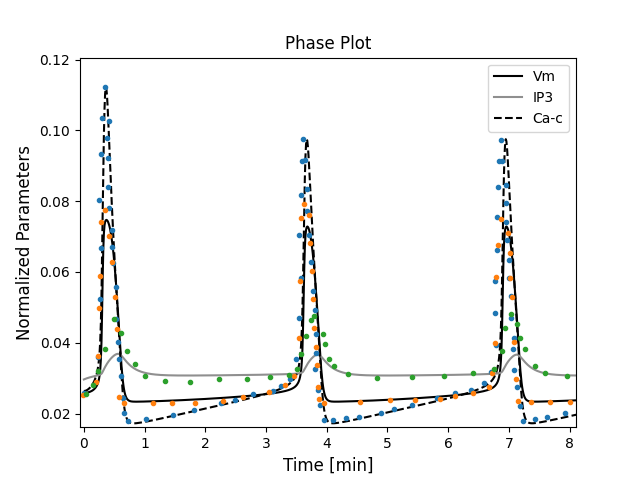
\includegraphics[width=1.0\linewidth]{Figure_2.png}
\caption{The primary data (*) of \cite[Figure 2A]{imtiaz2002theoretical} with our reproduction of all subfigures. To reproduce \cite[Figure 2A]{imtiaz2002theoretical}, use the Python manuscript \texttt{Fig2\_sim.py} and to plot it use \texttt{Plot\_Fig2.py}.}
\label{fig:fig2}
\end{figure}

\begin{figure}[ht!]%\centering
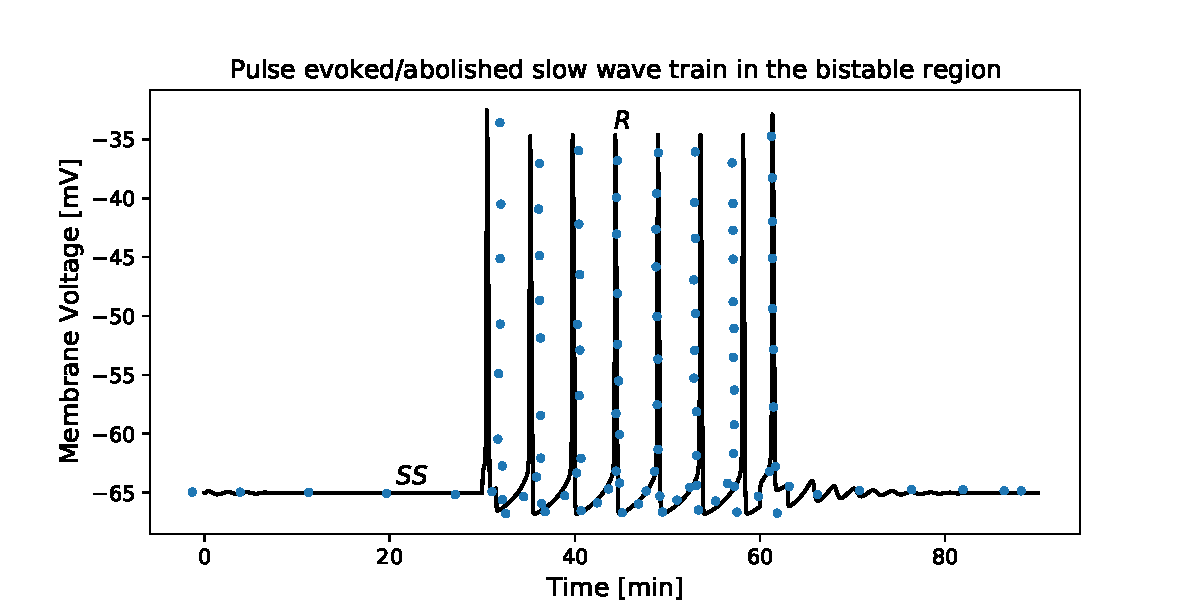
\includegraphics[width=1.0\linewidth]{Figure_3.pdf}
\caption{The primary data (*) of \cite[Figure 3A]{imtiaz2002theoretical} with our reproduction of all subfigures. To reproduce \cite[Figure 3A]{imtiaz2002theoretical}, use the Python script \texttt{Fig3\_sim.py} and to plot it use \texttt{Plot\_Fig3.py}.}
\label{fig:fig3}
\end{figure}

\begin{figure}[ht!]%\centering
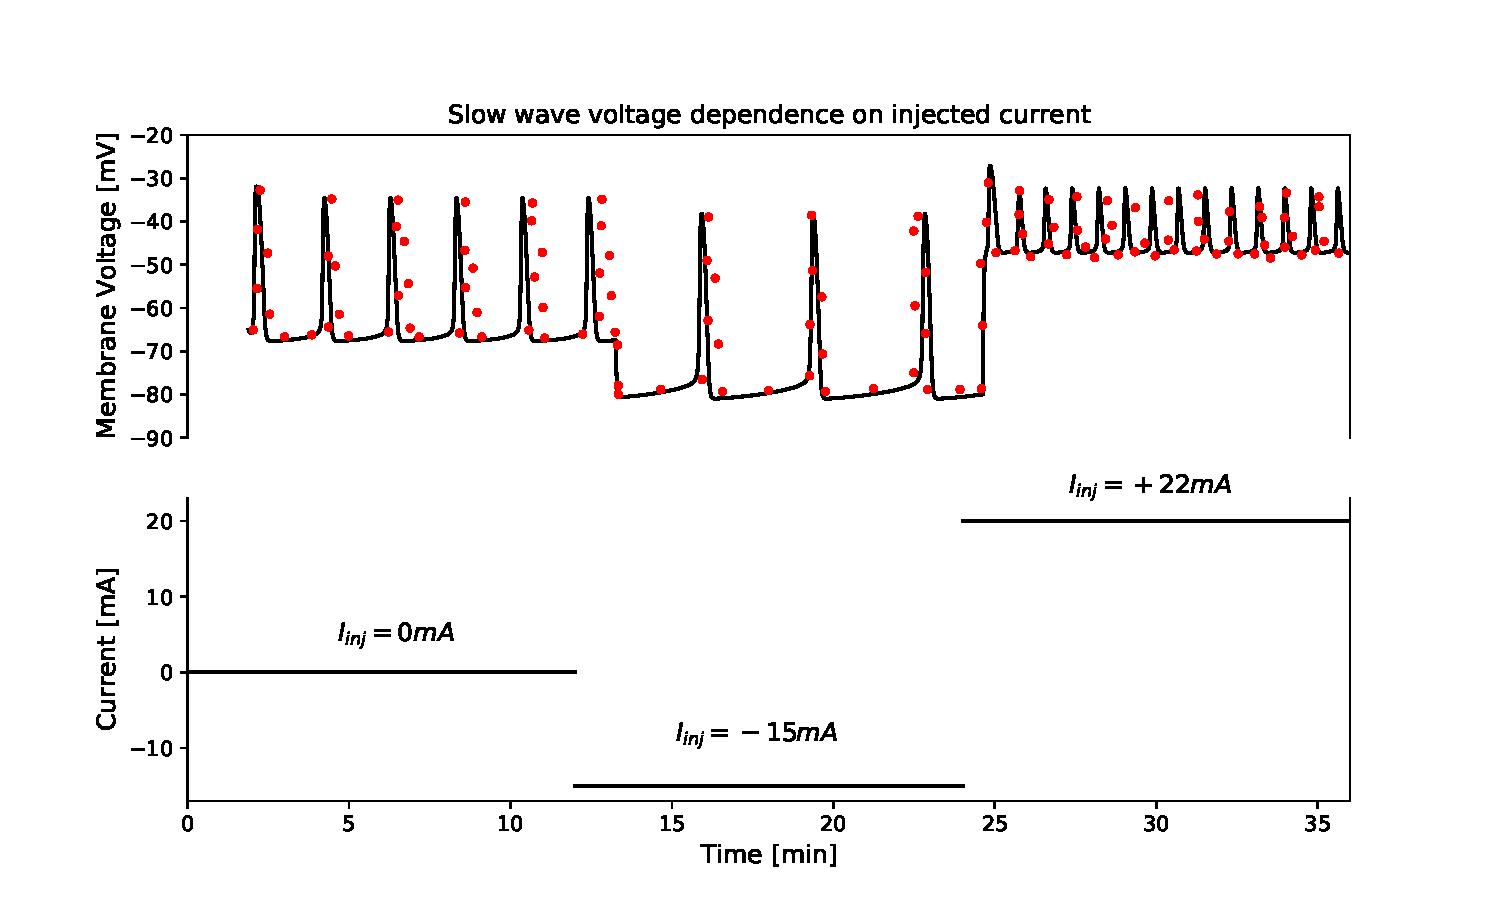
\includegraphics[width=1.0\linewidth]{Figure_4.pdf}
\caption{The primary data (*) of \cite[Figure 4A]{imtiaz2002theoretical} with our reproduction of all subfigures. To reproduce \cite[Figure 4A]{imtiaz2002theoretical}, use the Python script \texttt{Fig4\_sim.py} and to plot it use \texttt{Plot\_Fig4.py}.}
\label{fig:fig4}
\end{figure}

\begin{figure}[ht!]%\centering
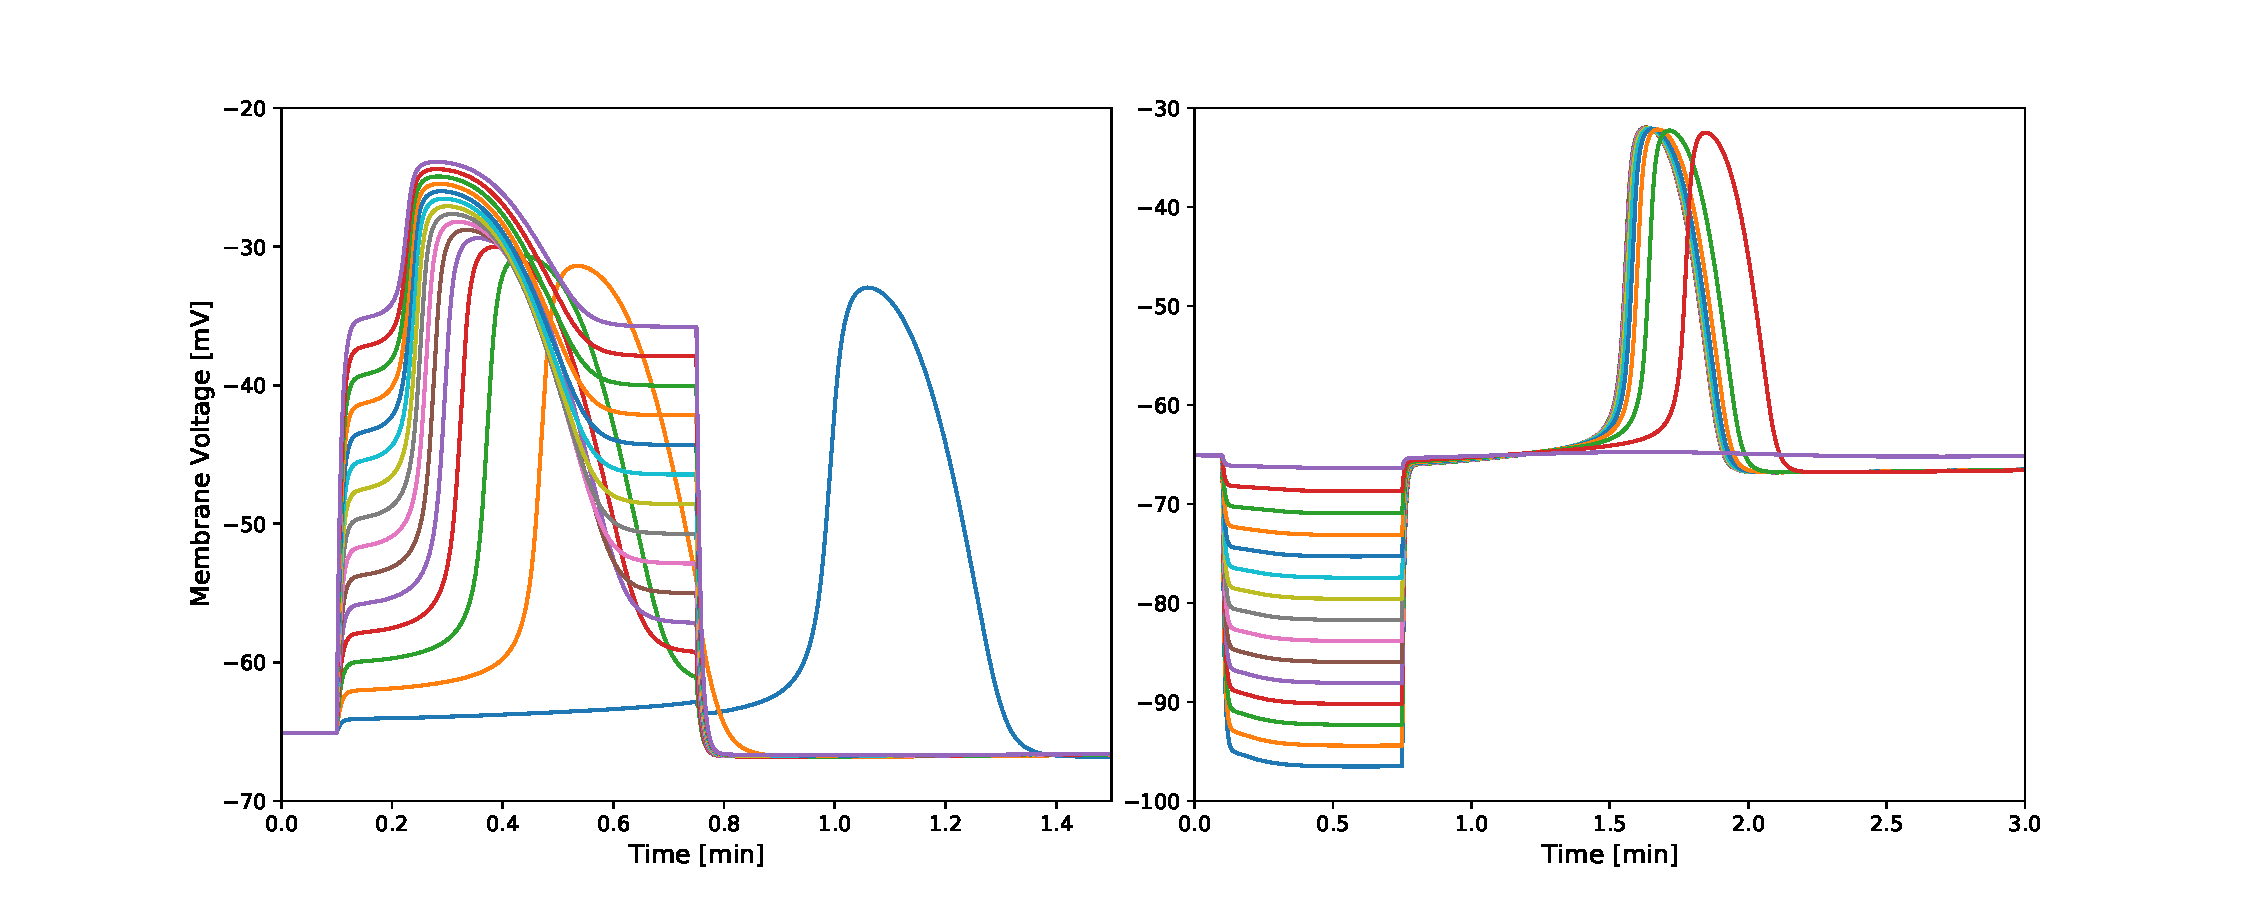
\includegraphics[width=1.0\linewidth]{Figure_6.pdf}
\caption{The primary data (*) of \cite[Figure 6(A and B)]{imtiaz2002theoretical} with our reproduction of all subfigures. To reproduce \cite[Figure 6(A and B)]{imtiaz2002theoretical}, use the Python script \texttt{Fig6\_sim.py} and to plot it use \texttt{Plot\_Fig6.py}.}
\label{fig:fig6}
\end{figure}

\begin{figure}[ht!]%\centering
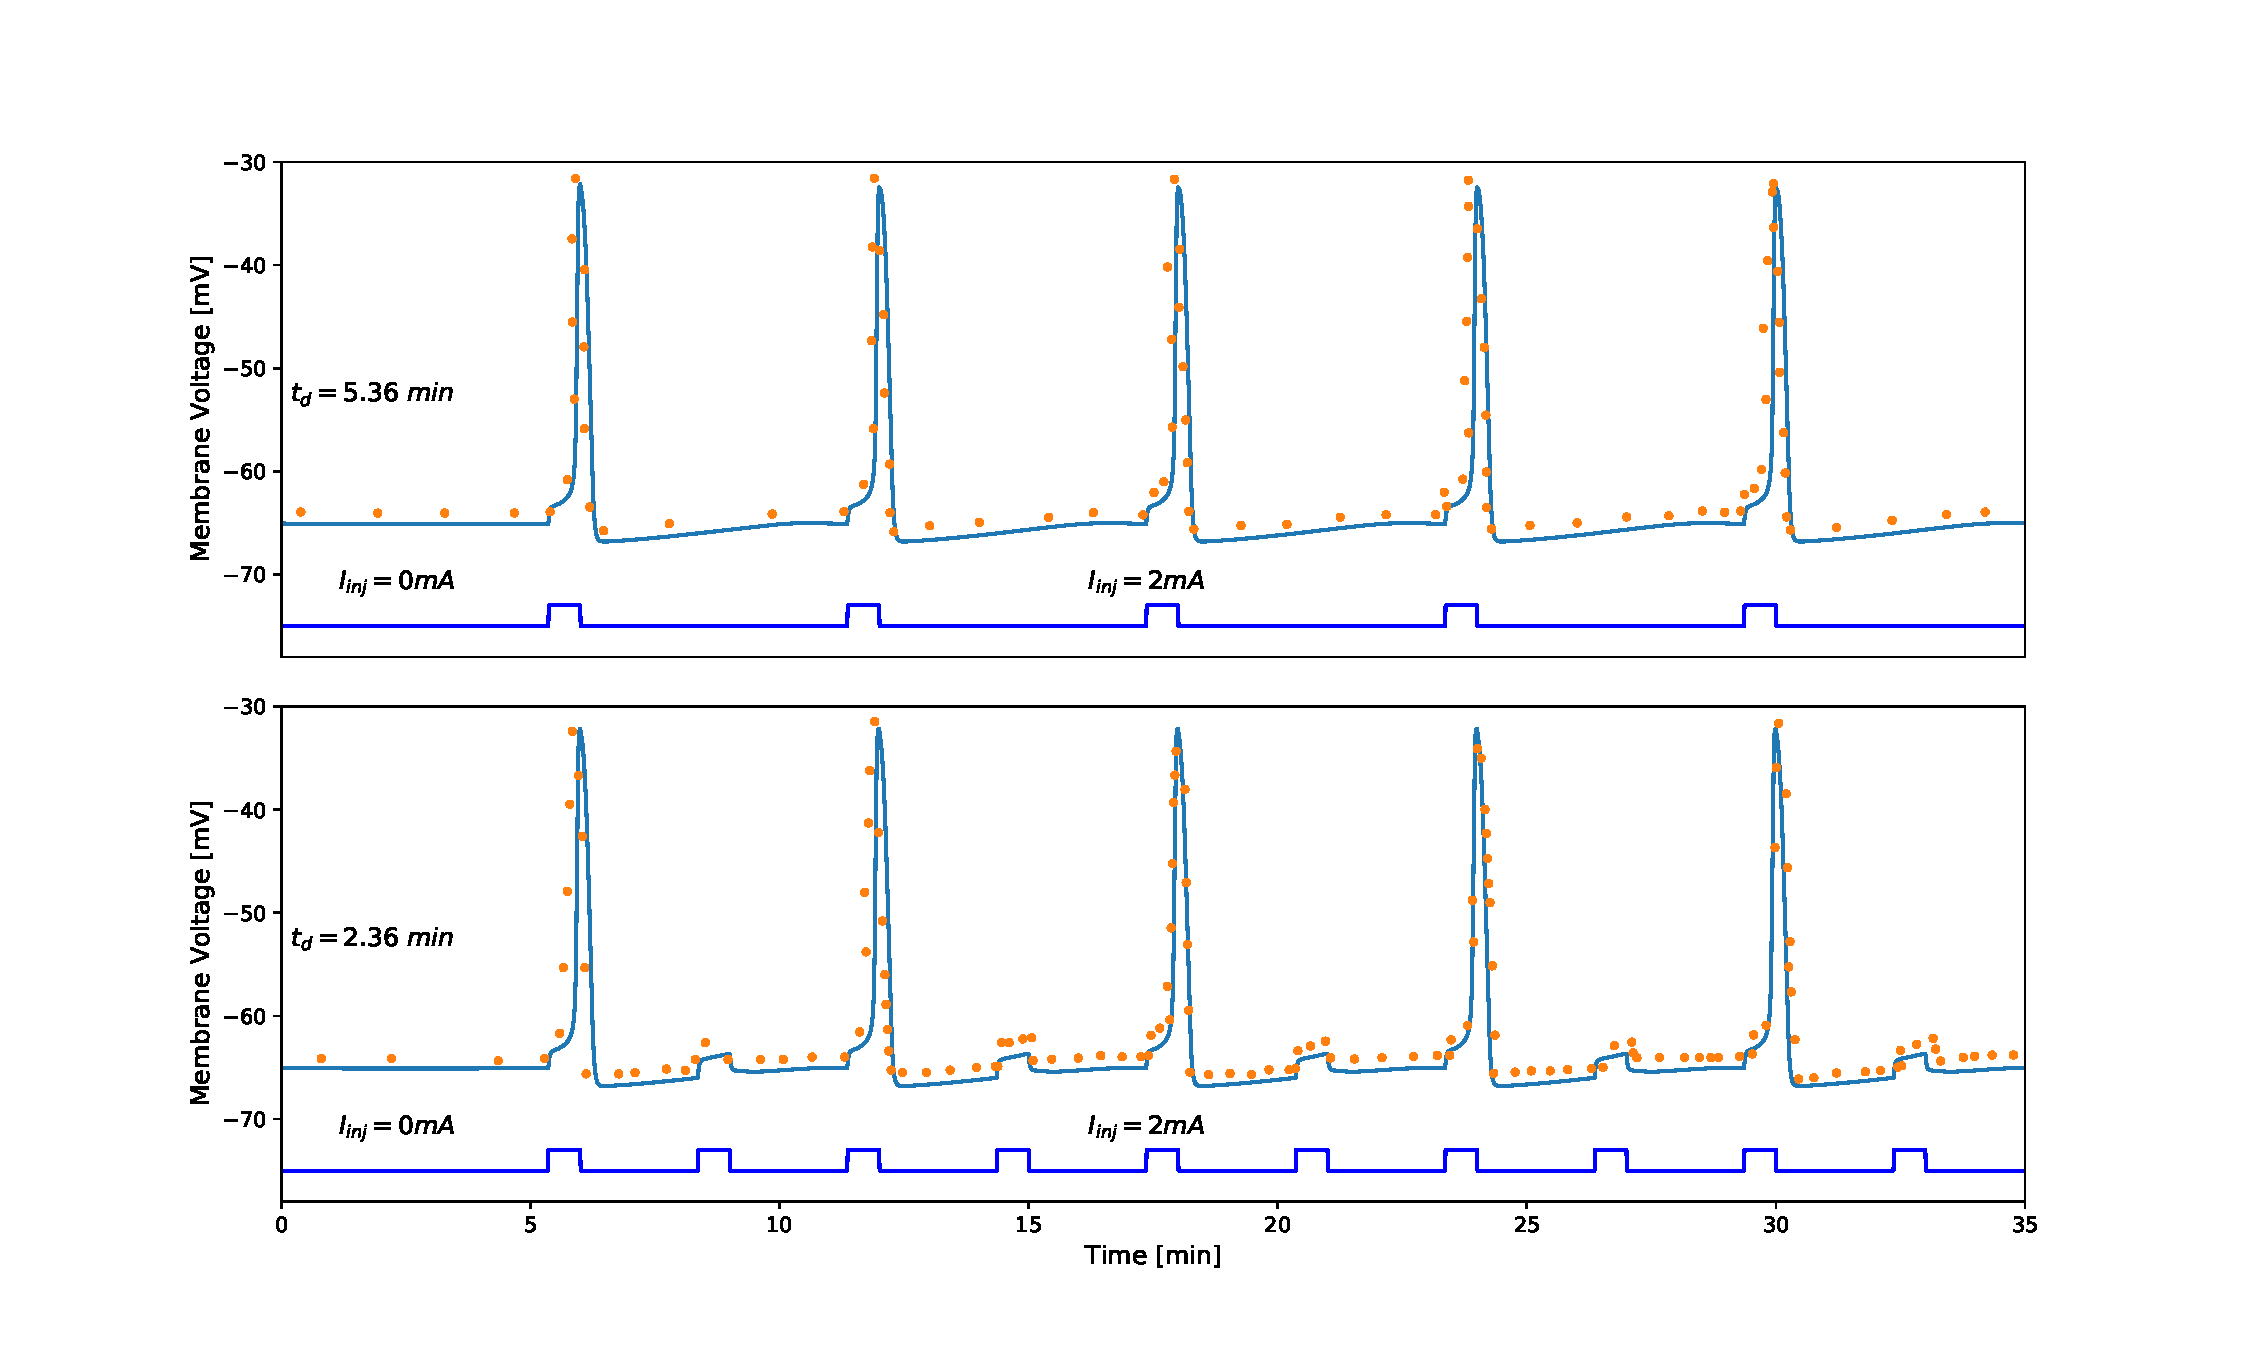
\includegraphics[width=1.0\linewidth]{Figure_8.pdf}
\caption{The primary data (*) of \cite[Figure 8A]{imtiaz2002theoretical} with our reproduction of all subfigures. To reproduce \cite[Figure 8A]{imtiaz2002theoretical}, use the Python script \texttt{Fig8\_sim.py} and to plot it use \texttt{Plot\_Fig8.py}.}
\label{fig:fig8}
\end{figure}
\section{Discussion}
We implemented the model of \cite{imtiaz2002theoretical} using CellML which can be reused in future. We successfully replicated simulation results and summarized detailed experiment settings for simulation in \autoref{Model Simulations}.
In doing this, we noticed trivial typographical errors in parameter units and references in \cite[Table 1, 3]{imtiaz2002theoretical}. Hence, we highlighted the issues and added correction to remove potential confusion in \autoref{Parameter_Values}.

\section{Acknowledgements}
The authors gratefully acknowledge the support of the Ministry of Business, Innovation and Employment’s
Catalyst Strategic Fund (12 Labours).

\bibliography{Ref}

\end{document}
